
\section{MTEX}


\begin{frame}{What is \MTEX: some numbers and facts}


\begin{block}{}

\begin{itemize}
\item developed since 2007
\item 37000 lines of matlab code in over 900 m-files
\item 20000 lines comments
\item 750 help pages
\item 5 reference papers
\item support for more than 20 pole figure and 5 EBSD data formats
\end{itemize}
\end{block}

\begin{block}{}
  \vspace*{0.25em}
  \hspace{1.25em}
  \begin{tabular}{ll}
    version & release date \\
    \toprule
    mtex 1.0 & June 2008 \\
    mtex 2.0 & October 2009 \\
    mtex 3.0 & August 2010 \\
    mtex 3.2 & September 2011\\
    mtex 3.3 & comming soon
  \end{tabular}
\end{block}


\end{frame}


\section{Live in 3d}

\subsection*{Vector3d}

\begin{frame}[fragile]
  \frametitle{Three dimensional vectors - The \MTEX Class \texttt{\bf vector3d}}

  Three dimensional vectors are given by there coordinate with respect to a
  orthogonal coordinate system $\vec X, \vec Y, \vec Z$
  \begin{equation*}
    \vec r = x \cdot \vec X + y \cdot \vec Y + z \cdot \vec Z
  \end{equation*}

  \pause

  \MTEX does not care about the coordinate system, but works only with the
  coordinates

  \begin{lstlisting}
r = vector3d(1,2,3)
  \end{lstlisting}

  \begin{columns}
    \begin{column}{8cm}
\begin{lstlisting}[style=output]
r = vector3d (show methods, plot)
  size: 1 x 1
  x y z
  1 2 3
\end{lstlisting}

      \pause
      \medskip

      The alignment of the coordinate system is only important when plotting
      data
      \begin{onlyenv}<3|handout>
\begin{lstlisting}
plotx2north
plot(r)
\end{lstlisting}
      \end{onlyenv}
      \begin{onlyenv}<4>
\begin{lstlisting}
plotx2east
plot(r)
\end{lstlisting}
      \end{onlyenv}

    \end{column}
    \begin{column}{3.5cm}
      \only<3|handout>{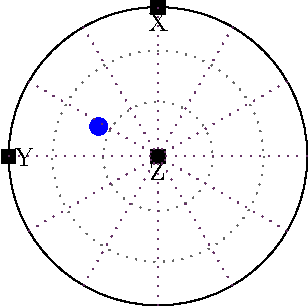
\includegraphics[width=3.5cm]{pic/vectorNorth}}
      \only<4>{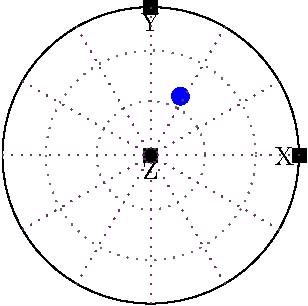
\includegraphics[width=3.5cm]{pic/vectorEast}}
    \end{column}
  \end{columns}

\end{frame}

\subsection*{Definition}

\begin{frame}[fragile,fragile,fragile]
  \frametitle{Defining vectors}

  polar coordinates: $\vec r = (\sin \theta \cos \rho,\sin \theta \sin \rho,\cos \theta)^{t}$

\begin{lstlisting}
r = vector3d('polar',theta,rho)
\end{lstlisting}

  \pause \medskip

  predefined vectors:
\begin{lstlisting}
r = xvector, r = yvector, r = zvector
\end{lstlisting}

  \pause \medskip

  importing vectors:
\begin{lstlisting}
r = loadVector3d('file','ColumnNames',{'x','y','z'})
\end{lstlisting}

  \pause \medskip

  combine vectors:
\begin{lstlisting}
r = [xvector, yvector, vector3d(1,1,1)];
\end{lstlisting}
\begin{lstlisting}[style=output]
r = vector3d (show methods, plot)
  size: 1 x 3
  x y z
  1 0 0
  0 1 0
  1 1 1
\end{lstlisting}

\pause \medskip

  index vectors:
\begin{lstlisting}
r(get(r,'x')>0)
\end{lstlisting}

\end{frame}

\subsection*{Calculations}

\begin{frame}[fragile]
  \frametitle{Vector Calculations}


  simple algebra:
\begin{lstlisting}
r = 2*xvector - yvector;
\end{lstlisting}

  \pause \medskip


  basic operations:
\begin{lstlisting}
dot(v1,v2)   % dot product
cross(v1,v2) % cross product
angle(v1,v2) % angle between two vectors
\end{lstlisting}

  \pause \medskip

  extract properties:
\begin{lstlisting}
theta = get(r,'theta')
rho   = get(r,'rho')
x = get(r,'x')
y = get(r,'y')
z = get(r,'z')
\end{lstlisting}

\end{frame}


\subsection*{Plotting}
\label{sec:plotting}

\begin{frame}[fragile]
  \frametitle{Plotting Vectors}

  \begin{columns}
    \begin{column}{8cm}
      spherical projections: \texttt{earea, edist, eangle, plain, 3d}
\begin{lstlisting}
plot(r,'projection','eangle')
\end{lstlisting}

      \pause \medskip

      hemisphere: \texttt{north, south, upper, lower}
\begin{lstlisting}
plot(r,'south')
\end{lstlisting}

      \pause \medskip

      combine plots:
\begin{lstlisting}
hold all
plot(vector3d(3,2,1));
hold off
\end{lstlisting}

      \pause \medskip

      contour plots:
\begin{lstlisting}
plot(r,'contourf')
\end{lstlisting}


    \end{column}
    \begin{column}{4cm}


      \includegraphics<1-2>[width=4cm]{pic/vectoreangle}

      \includegraphics<1-2>[width=4cm]{pic/vectorearea}

      \includegraphics<3-4>[width=4cm]{pic/vectorScatter}

      \includegraphics<4>[width=4cm]{pic/vectorContourAntipodal}
    \end{column}
  \end{columns}


\end{frame}



\subsection*{Annotations}

\begin{frame}[fragile]
  \frametitle{Add Annotations to Pole Figure Plots}


\begin{columns}
  \begin{column}{8.5cm}

\begin{overprint}
  \onslide<1|handout:0>%
  General Syntax:%
\begin{lstlisting}
annotate(vector,<options>)
\end{lstlisting}
  \onslide<2|handout:1>%
  General Syntax:
\begin{lstlisting}
annotate(orientation,<options>)
\end{lstlisting}
\end{overprint}

Options:
\begin{lstlisting}
Marker            % marker shape
MarkerSize        % marker size
MarkerFaceColor   % face color
MarkerEdgeColor   % edge color
label             % a label text
color, background % text colors
\end{lstlisting}

\begin{overprint}
  \onslide<1|handout:0>%
  Example:
\begin{lstlisting}
annotate([xvector,yvector,zvector],
 'Backgroundcolor','w','Marker','s',
 'MarkerEdgeColor','w','labeled',
 'MarkerFaceColor','k')
\end{lstlisting}

  \onslide<2|handout:1>
Example:
\begin{lstlisting}
annotate(q0,'label','$q_0$',...
   'marker','s','MarkerSize',4,...
   'MarkerFaceColor','r','color','b')
\end{lstlisting}

\end{overprint}

\end{column}

  \begin{column}{3.5cm}
    \begin{overlayarea}{3.5cm}{7cm}
      \onslide<1->
      \only<1|handout:0>{%
        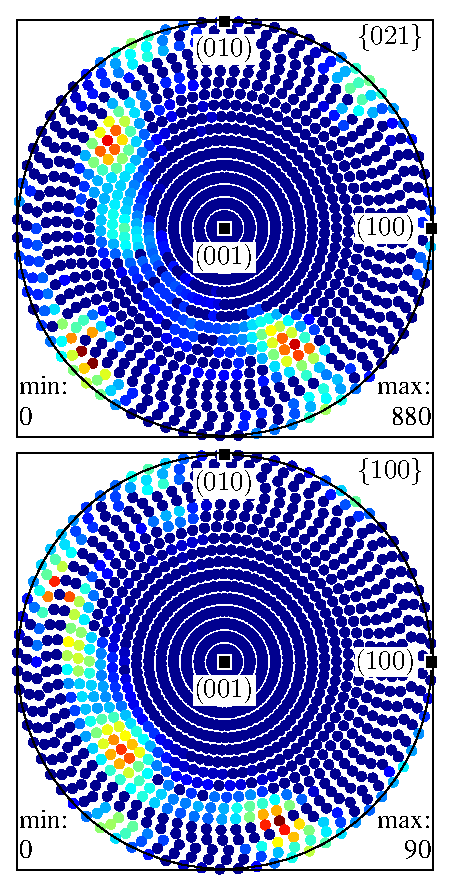
\includegraphics[width=3.5cm]{pic/annotationv}%
      }%
      \only<2>{%
        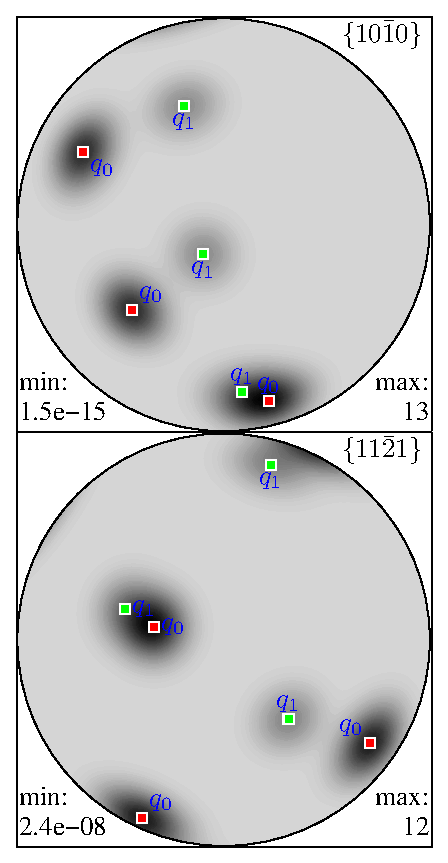
\includegraphics[width=3.5cm]{pic/annotationq}%
      }%
    \end{overlayarea}
  \end{column}

\end{columns}

\end{frame}

\subsection*{Axes}

\begin{frame}[fragile]
  \frametitle{Axes}

  Axes are three dimensional vectors where we do not care about length and
  direction, e.g. plane normals.

\begin{lstlisting}
r = vector3d(1,1,1,'antipodal')
\end{lstlisting}

\medskip
\pause

  This has effect on calculations, e.g. \texttt{angle, dot}
\begin{lstlisting}
angle(r,xvector)
\end{lstlisting}

\medskip
\pause

and plotting:

\begin{uncoverenv}<3>
  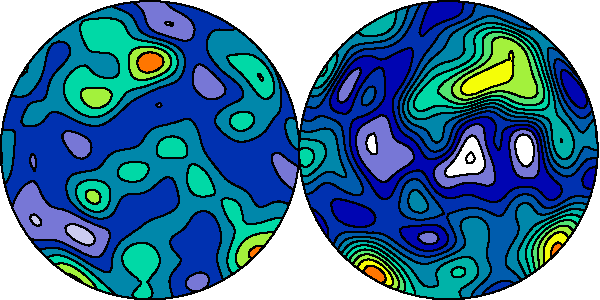
\includegraphics[width=7cm]{pic/vectorContour}
  \quad
  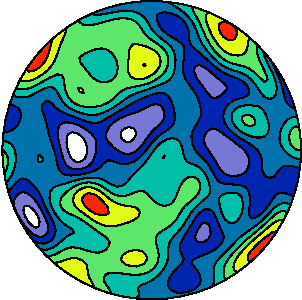
\includegraphics[width=3.5cm]{pic/vectorContourAntipodal}
\end{uncoverenv}


\end{frame}



%--------------------------------------------------------------------------------------------------------------------

\section{Rotations}

\subsection*{Basics}




\begin{frame}[fragile]
  \frametitle{Rotations - The \MTEX Class \texttt{\bf rotation}}

  A rotation is a transformation that maps a right handed coordinate system
  $(\vec X_{1}, \vec Y_{1}, \vec Z_{1})$ onto another right handed coordinate
  system $(\vec X_{2}, \vec Y_{2}, \vec Z_{2})$. It is given by the rotation
  matrix

  % \begin{equation*}
  %   \bf R = \left(
  %     \begin{matrix}
  %       \vec X_{1} \cdot \vec X_{2} & \vec Y_{1} \cdot \vec X_{2}& \vec Z_{1} \cdot \vec X_{2} \\
  %       \vec X_{1} \cdot \vec Y_{2} & \vec Y_{1} \cdot \vec Y_{2}& \vec Z_{1} \cdot \vec Y_{2} \\
  %       \vec X_{1} \cdot \vec Z_{2} & \vec Y_{1} \cdot \vec Z_{2}& \vec Z_{1} \cdot \vec Z_{2}
  %     \end{matrix}
  %   \right).
  % \end{equation*}
  \begin{equation*}
    \mathbf R = (\vec X_{2}, \vec Y_{2}, \vec Z_{2}) \cdot (\vec X_{1}, \vec Y_{1}, \vec Z_{1})^{t}
  \end{equation*}

  \medskip

  We have $\mathbf R \vec X_{1} = \vec X_{2}$, $\mathbf R \vec Y_{1} = \vec
  Y_{2}$ and $\mathbf R \vec Z_{1} = \vec Z_{2}$.

  \medskip
  \pause

  On the other hand, $\bf R$ transforms coordinates with respect to $(\vec
  X_{2}, \vec Y_{2}, \vec Z_{2})$ into coordinates with respect to $(\vec
  X_{1}, \vec Y_{1}, \vec Z_{1})$. I.e. for

  \begin{equation*}
    \vec r
    = x_{1} \vec X_{1} + y_{1} \vec Y_{1} + z_{1} \vec Z_{1}
    = x_{2} \vec X_{2} + y_{2} \vec Y_{2} + z_{2} \vec Z_{2}
  \end{equation*}

  we have

  \begin{equation*}
    \mathbf R
    \left(
      \begin{matrix}
        x_{2}\\
        y_{2}\\
        z_{2}
      \end{matrix}\right)
    = \left(
      \begin{matrix}
        x_{1}\\
        y_{1}\\
        z_{1}
      \end{matrix}\right)
  \end{equation*}

\end{frame}



\subsection*{Euler Angles}
\label{sec:euler-angles}

\begin{frame}[fragile]
  \frametitle{Euler Angles}

  Most commonly, rotations are given by Euler angles.

  \begin{lstlisting}
R = rotation('Euler',10*degree,20*degree,30*degree)
  \end{lstlisting}
  \begin{onlyenv}<1>
  \begin{lstlisting}[style=output]
R = rotation (show methods, plot)
  size: 1 x 1

  Bunge Euler angles in degree
  phi1  Phi phi2
    10   20   30
  \end{lstlisting}
  \end{onlyenv}

  \pause

  \begin{lstlisting}
R = rotation('Euler',...
    10*degree,20*degree,30*degree,'Roe')
  \end{lstlisting}
  \begin{onlyenv}<2>
  \begin{lstlisting}[style=output]
R = rotation (show methods, plot)
  size: 1 x 1

  Bunge Euler angles in degree
  phi1  Phi phi2
   100   20  300
  \end{lstlisting}
\end{onlyenv}

\pause

Supported conventions are \texttt{Bunge}, \texttt{Matthies}, \texttt{Roe},
\texttt{Kocks}, \texttt{Canova}.
  \begin{lstlisting}
setpref('mtex','EulerAngleConvention','Roe')
  \end{lstlisting}

  \begin{onlyenv}<3>
  \begin{lstlisting}[style=output]
R = rotation (show methods, plot)
  size: 1 x 1

  Roe Euler angles in degree
  Psi Theta   Phi
   10    20    30
 \end{lstlisting}
\end{onlyenv}
\end{frame}

\subsection*{Axis Angle Representation}
\label{sec:axis-angle-repr}

\begin{frame}[fragile]
  \frametitle{Other Ways to Define a Rotation}

  A rotation is uniquely defined by its rotation axis and its rotation angle

  \begin{lstlisting}
R = rotation('axis',xvector,'angle',45*degree)
  \end{lstlisting}

  \pause
  \medskip

  Conversely, one can compute axis / angle from a rotation

  \begin{lstlisting}
get(R,'axis'), get(R,'angle')
  \end{lstlisting}

  \pause
  \medskip

Given four vectors $\vec u_{1}, \vec u_{2}, \vec v_{1}, \vec v_{2}$ there is a
unique rotation $\mathbf R$ such that  $\mathbf R \vec u_{1} = \vec v_{1}$ and
$\mathbf R \vec u_{2} = \vec v_{2}$:

\begin{lstlisting}
R = rotation('map',u1,v1,u2,v2)
\end{lstlisting}

  \pause
  \medskip

Of course one can also define a rotation by its $3 \times 3$ matrix

  \begin{lstlisting}
R = rotation('matrix',A)
  \end{lstlisting}

or by quaternions

  \begin{lstlisting}
R = rotation('quaternion',a,b,c,d)
  \end{lstlisting}

\end{frame}


\subsection*{Basic Calculations}
\label{sec:euler-angles}

\begin{frame}[fragile]
  \frametitle{Basic Calculations}

  \begin{columns}
    \begin{column}{8cm}

  rotate a vector:
\begin{lstlisting}
v = R * v
\end{lstlisting}

  \pause \medskip

the inverse rotation:
\begin{lstlisting}
inverse(R)
\end{lstlisting}

  \pause \medskip

  combine rotations:
\begin{lstlisting}
R = R1 * R2
\end{lstlisting}

  \pause \medskip

  plotting:
\begin{lstlisting}
plot(R)           % plot new
plot(R,'scatter') % Rodriguez space
\end{lstlisting}

    \end{column}

    \begin{column}{3.7cm}
      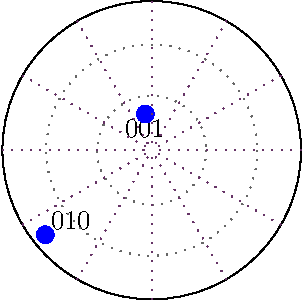
\includegraphics[width=3.7cm]{pic/rotationNorth}

      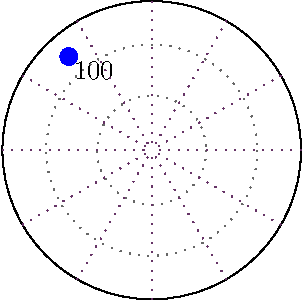
\includegraphics[width=3.7cm]{pic/rotationSouth}
    \end{column}

  \end{columns}

\end{frame}


\section{Symmetries}
\label{sec:symmetries}

\subsection*{Crystal Symmetries}
\label{sec:crystal-symmetries}


\begin{frame}[fragile,fragile]
  \frametitle{Crystal Geometry}


  \begin{columns}
    \begin{column}{8cm}
      All the rotations $\mathbf R$ that keeps the crystal lattice invariant
      form the so called \alert{point group} of the crystal.

\begin{lstlisting}
C = symmetry('mmm')
\end{lstlisting}
    \begin{onlyenv}<1>
\begin{lstlisting}[style=output]
C = crystal symmetry (show methods, plot)

  symmetry: mmm (mmm)
  a, b, c : 1, 2, 3
\end{lstlisting}
    \end{onlyenv}

    \pause \medskip

    import data from crystal information files
\begin{lstlisting}
C = symmetry('Quarz.cif')
\end{lstlisting}
    \begin{onlyenv}<2>
\begin{lstlisting}[style=output]
C = crystal symmetry (show methods, plot)

  mineral           : Quartz
  symmetry          : P 32 2 1 (-3m)
  a, b, c           : 4.9, 4.9, 5.4
  alpha, beta, gamma: 90°, 90°, 120°
  reference frame   : X||a*, Y||b, Z||c*
\end{lstlisting}
    \end{onlyenv}

  \end{column}
  \begin{column}{3.7cm}
      \includegraphics<1>[width=3.7cm]{pic/mmmNorth}

      \includegraphics<1>[width=3.7cm]{pic/mmmSouth}

      \includegraphics<2>[width=3.7cm]{pic/symmetryNorth}

      \includegraphics<2>[width=3.7cm]{pic/symmetrySouth}
  \end{column}
\end{columns}
\end{frame}

\subsection*{Crystal Symmetries}
\label{sec:crystal-symmetries}


\begin{frame}[fragile]
  \frametitle{Crystal Geometry}

  The unit cell of a crystal is specified by the length of its three edges
  $\vec a, \vec b, \vec c$ and by angles $\alpha, \beta, \gamma$ they enclose

  \begin{lstlisting}
C = symmetry('triclinic',[a b c],[alpha beta gamma])
  \end{lstlisting}

  \begin{columns}
    \begin{column}{7.5cm}

      \begin{uncoverenv}<2->
        The axes of the reciprocal lattice are defined to be orthogonal to $\vec a,
        \vec b, \vec c$, i.e.

\begin{equation*}
  \vec a^{*} = \vec b \times \vec c, \;
  \vec b^{*} = \vec c \times \vec a, \;
  \vec c^{*} = \vec a \times \vec b
\end{equation*}
      \end{uncoverenv}



      \begin{uncoverenv}<3->
        For comparison with the specimen coordinate system one needs also an
        orthogonal coordinate system to be inscribed into $(\vec a, \vec b,
        \vec c)$.  \alert{There are different conventions:}
      \end{uncoverenv}


    \end{column}

    \begin{column}{4.5cm}
      \begin{tikzpicture}[x  = {(-0.5cm,-0.5cm)},
        y  = {(0.9659cm,-0.25882cm)},
        z  = {(0cm,1cm)},
        scale = 2]

\draw[draw=green, dashed] (0,0,0) -- (1.2,0,0) -- (1,1,0) -- (-0.2,1,0) --
(0,1.2,1) -- (0.2,0.2,1) --  (1.4,0.2,1) -- (1.2,0,0);

\draw[draw=green, dashed] (0,1.2,1) -- (1.2,1.2,1) -- (1,1,0);
\draw[draw=green, dashed] (1.2,1.2,1) -- (1.4,0.2,1);


\draw[draw=green,very thick] (0,0,0) -- (1.2,0,0) node [anchor=north,color=green!70!black] {$\vec a$};
\draw[draw=green,very thick] (0,0,0) -- (-0.2,1,0) node [anchor=west,color=green!70!black] {$\vec b$};
\draw[draw=green,very thick] (0,0,0) -- (0.2,0.2,1) node[anchor=south,color=green!70!black] {$\vec c$};

\only<1>{
\draw[draw=green] (0.3,0,0) arc (250:329:0.3cm);% node {$\alpha$};
\draw[draw=green] (-0.03,0.2,0) arc (0:68:0.3cm);% node {$\alpha$};
\draw[draw=green] (0.3,0,0) arc (200:112:0.3cm);% node {$\alpha$};
\node at (0.15,0.01,0.1)[color=green!70!black]{$\beta$};
\node at (0.01,0.15,0.1)[color=green!70!black]{$\alpha$};
\node at (0.15,0.1,0)[color=green!70!black]{$\gamma$};
}


\only<2->{
\draw[->,draw=red,very thick] (0,0,0) -- (0,0,1.2) node [anchor=west,color=red!70!black] {$\vec c^{*}$};
\draw[->,draw=red,very thick] (0,0,0) -- (1,0.2,-0.24) node [anchor=west,color=red!70!black] {$\vec a^{*}$};
\draw[->,draw=red,very thick] (0,0,0) -- (0,1.2,-0.24) node [anchor=north,color=red!70!black] {$\vec b^{*}$};
}

\only<3|handout>{
\draw[->,draw=black,ultra thick] (0,0,0) -- (1,0,0) node
[anchor=north,color=black] {$\vec{\mathbf x}$};
\draw[->,draw=black,ultra thick] (0,0,0) -- (0,1,0) node
[anchor=north,color=black] {$\vec{\mathbf y}$};
\draw[->,draw=black,ultra thick] (0,0,0) -- (0,0,1) node
[anchor=east,color=black] {$\vec{\mathbf z}$};
}

\only<4>{
\draw[->,draw=black,ultra thick] (0,0,0) -- (1,0.2,0) node
[anchor=north,color=black] {$\vec{\mathbf x}$};
\draw[->,draw=black,ultra thick] (0,0,0) -- (-0.2,1,0) node
[anchor=north,color=black] {$\vec{\mathbf y}$};
\draw[->,draw=black,ultra thick] (0,0,0) -- (0,0,1) node
[anchor=east,color=black] {$\vec{\mathbf z}$};
}

\end{tikzpicture}

\end{column}
\end{columns}

\begin{onlyenv}<3|handout>
  \begin{lstlisting}
C = symmetry('trigonal',[a b c],'X||a','Z||c*')
  \end{lstlisting}
\end{onlyenv}

\begin{onlyenv}<4>
  \begin{lstlisting}
C = symmetry('trigonal',[a b c],'X||b','Z||c*')
  \end{lstlisting}
\end{onlyenv}

\end{frame}


\section{Miller Indices}
\label{sec:miller-indices}


\subsection*{definition}
\label{sec:definition}


\begin{frame}[fragile]
  \frametitle{Miller Indices}

  \begin{columns}
    \begin{column}{5.8cm}

A direction with respect to the crystal coordinate system \alert{S}:
\begin{equation*}
  \vec r = u \cdot \vec a+ v \cdot \vec b + w \cdot \vec c.
\end{equation*}
\begin{lstlisting}
r = Miller(u,v,w,S,'uvw')
\end{lstlisting}

\medskip
\pause

A direction in reciprocal coordinates
\begin{equation*}
  \vec r = h \cdot \vec a^{*}+ k \cdot \vec b^{*} + \ell \cdot \vec c^{*}.
\end{equation*}
\begin{lstlisting}
r = Miller(h,k,l,S,'hkl')
\end{lstlisting}

\pause
\medskip

A direction in the orthogonal coordinate system
\begin{lstlisting}
r = Miller(xvector,S)
\end{lstlisting}

    \end{column}
    \begin{column}{5.7cm}

      \begin{center}
        \includegraphics<1>[width=4.5cm]{pic/MillerUVW}
        \includegraphics<2>[width=4.5cm]{pic/MillerHKL}
        \includegraphics<3>[width=4.5cm]{pic/MillerPlane}
      \end{center}

      \begin{lstlisting}
S = symmetry('3',[1 1 4])
  \end{lstlisting}
  \begin{onlyenv}<1|handout>
  \begin{lstlisting}
m = Miller(1,1,1,S,'uvw')
plot(m,'labeled')
  \end{lstlisting}
  \end{onlyenv}
  \begin{onlyenv}<2>
   \begin{lstlisting}
m = Miller(1,1,1,S,'hkl')
plot(m,'labeled')
   \end{lstlisting}
 \end{onlyenv}
 \begin{onlyenv}<3>
   \begin{lstlisting}
m = Miller(1,1,1,S,'hkl')
plot(m,'plane')
   \end{lstlisting}
  \end{onlyenv}
\end{column}
  \end{columns}

\end{frame}

\subsection*{Calculations}

\begin{frame}[fragile]
  \frametitle{Calculations}

   \begin{columns}
     \begin{column}{8cm}
        Find all symmetrically equivalent directions
        \begin{lstlisting}
symmetrise(m)
        \end{lstlisting}

      \begin{onlyenv}<1->
        \begin{lstlisting}[style=output]
ans = Miller (show methods, plot)
  size: 6 x 1
  options: uvw
  symmetry: 3m, X||a*, Y||b, Z||c*
  u  1 -2  1  1 -2  1
  v  1  1 -2 -2  1  1
  t -2  1  1  1  1 -2
  w  1  1  1 -1 -1 -1
       \end{lstlisting}
     \end{onlyenv}

        \pause
        \medskip

        Plot all symmetrically equivalent directions
        \begin{lstlisting}
plot(m,'symmetrised','labeled')
        \end{lstlisting}

        \pause
        \medskip

        Compute angle modulo symmetry
  \begin{lstlisting}
angle(m1,m2) / degree
  \end{lstlisting}

     \end{column}
     \begin{column}{4cm}
       \includegraphics<1->[width=4cm]{pic/MillerSymmetrised}%\\
%       \includegraphics<1->[width=4cm]{pic/Symmetry}
     \end{column}
   \end{columns}

\end{frame}

\section{Orientations}
\label{sec:orientations}

\subsection*{Definition}

\begin{frame}

\frametitle{Crystal Orientations}

  \begin{columns}

    \begin{column}{6.3cm}

      The \alert{orientation} of a crystal is the class of rotations $[\mathbf
      R]$ that maps the specimen coordinate system $\vec X, \vec Y, \vec Z$
      onto one of the crystallographic equivalent orthogonal crystal
      coordinate systems $\vec x, \vec y, \vec z$.
      %\pause
      Let
      \begin{equation*}
        \vec v = r_{1} \vec X + r_{2} \vec Y + r_{3} \vec Y
               = h_{1} \vec x + h_{2} \vec y + h_{3} \vec z.
      \end{equation*}
      Then
      \begin{equation*}
        \left(
        \begin{matrix}
          r_{1}\\r_{2}\\r_{3}
        \end{matrix}
        \right)
        =
        \mathbf S_{S} \mathbf R \mathbf S_{C}
                \left(
        \begin{matrix}
          h_{1}\\h_{2}\\h_{3}
        \end{matrix}
        \right).
      \end{equation*}

      %\pause

      \alert{Orientations transform crystal coordinates into specimen coordinates.}

    \end{column}

    \begin{column}{5cm}

      \begin{tikzpicture}[scale=0.5]

        \draw[->, >=latex, color=green!80, thick] (0,0) -- (0,12) node[left] {$\vec Z$};
        \draw[->, >=latex, color=green!80, thick] (0,0) -- (6,0) node[right] {$\vec Y$};
        \draw[->, >=latex, color=green!80, thick] (0,0) -- (-2,-2) node[left] {$\vec X$};
%        \draw (6,11) node[color=green]{$K_S$};

        \foreach \xpos/\ypos/\xx/\xy/\yx/\yy/\zx/\zy
        in {
0.20/1.63/-0.20/0.13/1.09/0.10/-0.31/-2.21,
3.11/7.11/0.80/0.87/-0.20/0.55/1.50/-0.90,
3.70/4.70/-0.03/0.87/0.36/-0.55/-2.12/-0.90,
-1.91/1.15/-0.81/-0.59/0.59/-0.81/-1.00/-1.00,
2.90/9.73/-0.06/0.62/-1.11/-0.17/-0.22/-1.83,
%-0.67/6.44/-0.86/0.34/0.59/1.05/0.81/-0.37,
%1.13/9.19/-0.79/-0.78/0.37/-0.79/-1.40/0.21,
%2.28/0.74/0.44/1.02/-0.70/0.43/1.50/0.28,
%0.70/0.07/-0.06/1.08/-0.83/-0.25/1.50/0.28,
3.81/2.27/1.04/0.35/-0.40/0.54/-0.22/-1.83,
%-1.71/7.06/-0.16/0.06/0.61/1.04/1.85/-0.81,
%3.37/1.43/-0.61/-0.60/0.93/-0.23/-0.22/-1.83,
%-0.49/9.19/0.24/0.73/0.27/0.84/-2.12/0.28,
-1.21/9.29/1.07/-0.04/0.29/0.64/-0.22/-1.83,
%2.21/8.17/1.01/0.53/0.27/0.34/0.81/-1.85,
-0.74/3.46/-0.93/-0.71/0.05/0.48/-1.23/1.43,
-1.51/8.21/-0.68/-0.33/-0.53/-0.87/-1.43/1.23,
%1.37/1.83/1.07/0.51/-0.29/0.99/-0.22/0.21,
0.25/6.41/0.24/1.01/0.90/-0.27/-1.23/-0.81,
0.23/-1.12/-0.77/-0.57/0.31/-0.95/1.50/0.28
        }
        \fillcrystal{\xpos,\ypos}{\xx,\xy}{\yx,\yy}{\zx,\zy}{color=red};

      \end{tikzpicture}
    \end{column}
\end{columns}
\end{frame}


\subsection*{Defining Orientations}
\label{sec:defin-orient}

\begin{frame}[fragile]
  \frametitle{Defining Orientations}

  define orientations by Euler angles:
  \begin{lstlisting}
CS = symmetry('-3m');
SS = symmetry('triclinic')
O  = orientation('Euler',10*degree,5*degree,0,CS,SS)
  \end{lstlisting}
  \begin{onlyenv}<1>
  \begin{lstlisting}[style=output]
O = orientation (show methods, plot)
  size: 1 x 1
  crystal symmetry: 3m, X||a*, Y||b, Z||c*
  sample symmetry : triclinic

  Roe Euler angles in degree
  Psi Theta   Phi
   10     5     0
  \end{lstlisting}
  \end{onlyenv}

  \pause
  import orientations:
  \begin{lstlisting}
O  = loadOrientation('filename','CS',CS,'SS',SS,...
'ColumnNames',{'phi1','Phi','phi2'})
  \end{lstlisting}
  \begin{onlyenv}<2>
  \begin{lstlisting}[style=output]
O = orientation (show methods, plot)
  size: 1000 x 1
  crystal symmetry: 3m, X||a*, Y||b, Z||c*
  sample symmetry : triclinic
  \end{lstlisting}
  \end{onlyenv}

\pause

define orientations by Miller indices:
   \begin{lstlisting}
O  = orientation('Miller',[h k l],[u,v,w],CS,SS)
  \end{lstlisting}

\pause

standard orientations: \texttt{Cube, CubeND22, CubeND45, CubeRD, Goss,
invGoss, Copper, Copper2, SR, SR2, SR3, SR4, Brass, Brass2, PLage, PLage2,
QLage, QLage2, QLage3, QLage4}

\begin{lstlisting}
O  = brassOrientation(CS,SS)
\end{lstlisting}

\end{frame}


\subsection*{Calculating with Orientations}
\label{sec:calc-with-orient}

\begin{frame}[fragile,fragile,fragile,fragile]
  \frametitle{Calculating with Orientations}

  find all symmetrically equivalent:
\begin{lstlisting}
symmetrise(O)
\end{lstlisting}
  \begin{onlyenv}<1>
\begin{lstlisting}[style=output]
ans = rotation (show methods, plot)
  size: 6 x 1

  Roe Euler angles in degree
  Psi Theta   Phi
   10     5     0
   10     5   120
   10     5   240
  190   175    60
  190   175   180
  190   175   300
\end{lstlisting}
  \end{onlyenv}


  \pause
  \medskip

  convert crystal into specimen coordinates:
\begin{lstlisting}
h = Miller(1,0,0,CS);
r = O * h
\end{lstlisting}

  \pause
  \medskip

  convert specimen into crystal coordinates:
\begin{lstlisting}
r = xvector
h = inverse(O) * r
\end{lstlisting}

  \pause
  \medskip

  change specimen coordinates:
  \begin{lstlisting}
R  = rotation('axis',zvector,'angle',90*degree)
O2 = R * O1
\end{lstlisting}

\end{frame}


\subsection*{Misorientations}
\label{sec:orientations}

\begin{frame}[fragile]

  \frametitle{Misorientations}

  The \alert{Misorientation} between two crystals is the rotation that brings
  the corresponding coordinate systems in coincidence:

\begin{lstlisting}
MO = inverse(O1) * O2
\end{lstlisting}

\begin{onlyenv}<1>
\begin{lstlisting}[style=output]
MO = misorientation (show methods, plot)
  size: 1 x 1
  crystal symmetry: Quartz (P 32 2 1, X||a*, Y||b, Z||c*)
  crystal symmetry: Fe (m-3m)

  Roe Euler angles in degree
      Psi   Theta     Phi
  2.58238 56.6839  73.197
\end{lstlisting}
\end{onlyenv}


  \pause
  \medskip

  compute misorientation angle modulo symmetry
\begin{lstlisting}
angle(O1,O2) / degree, angle(MO) /degree
\end{lstlisting}

  \pause
  \medskip

  compute the misorientation axis
\begin{lstlisting}
axis(MO)
\end{lstlisting}

  \begin{onlyenv}<3>
\begin{lstlisting}[style=output]
ans = Miller (show methods, plot)
  size: 1 x 1
  symmetry: C2
  h -2
  k  3
  l  9
\end{lstlisting}
  \end{onlyenv}


\end{frame}


% \begin{frame}[fragile]
% \begin{lstlisting}[mathescape=true]
% rot = rotation('Euler',$\phi_1$,$\Phi$,$\phi_2$,'ZXZ')
% rot = rotation('Euler',$\alpha$,$\beta$,$\gamma$,'ABG')
% rot = rotation('axis',v,'angle',omega)
% rot = rotation('map',$u_1$, $v_1$, $u_2$, $v_2$) % $\mathbf{gu}_1=\mathbf{v}_1,\mathbf{gu}_2=\mathbf{v}_2$
% \end{lstlisting}

% \begin{columns}
%   \begin{column}{8.5cm}

%     Calculations:

% \begin{lstlisting}
% v = rot * u    % apply rot to u
% rot = rot1 * rot2
% \end{lstlisting}

%     Basic Functions:

% \begin{lstlisting}[mathescape=true]
% angle(rot), axis(rot)
% angle(rot1,rot2), inverse(rot)
% [$\phi_1$,$\Phi$,$\phi_2$] = Euler(rot)
% [$\alpha$,$\beta$,$\gamma$] = Euler(rot,'ABG')
% \end{lstlisting}

%   \end{column}

%   \begin{column}{3cm}
%     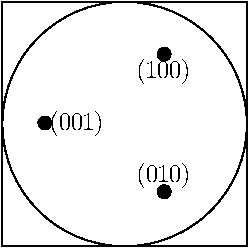
\includegraphics[width=3cm]{pic/quaternion}
%   \end{column}

% \end{columns}
% \end{frame}


% \subsection*{Symmetry}
% \begin{frame}[fragile]
%   \frametitle{Crystal Symmetries - The \MTEX Class \texttt{\bf symmetry}}

%   Definition:

% \begin{lstlisting}
% S = symmetry('triclinic',[a,b,c],[alpha,beta,gamma])
% S = symmetry('-3m',[a,b,c],/+'X||a*'+/);
% S = symmetry('-3m',[a,b,c],'X||a','Z||c*');
% S = symmetry('O');
% \end{lstlisting}

% \medskip

% \begin{columns}
%   \begin{column}{8.5cm}

% Load Symmetry from CIF file:

% \begin{lstlisting}
% symmetry('quartz.cif')
% \end{lstlisting}

% \medskip

%     Basic Functions:

% \begin{lstlisting}
% symmetrise(v,S)
% symmetrise(rot,CS,SS)
% rotation(S)
% project2FundamentalRegion(v,CS)
% project2FundamentalRegion(rot,CS,SS)
% \end{lstlisting}
%   \end{column}

%   \begin{column}{3cm}
%     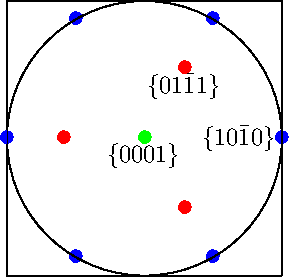
\includegraphics[width=3cm]{pic/sym}
%   \end{column}

% \end{columns}

% \end{frame}

% \subsection*{Miller}

% \begin{frame}[fragile]
%   \frametitle{Crystal Directions - The \MTEX Class \texttt{\bf Miller}}

%   Definition:

% \begin{lstlisting}
% m = Miller(u,v,w,CS,'uvw');
% m = Miller(h,k,i,l,CS,'hkl');
% m = [Miller(1,1,-2,3,CS),Miller(0,1,-1,0,CS)]
% \end{lstlisting}

% \medskip

% \begin{columns}
%   \begin{column}{8.5cm}

%     Calculations:

% \begin{lstlisting}
% h1 + h2
% rot * h     % apply rot on h
% \end{lstlisting}

%     \medskip

%     Basic Functions:

%     \begin{onlyenv}<1>
% \begin{lstlisting}
% eq(h1,h2), angle(h1,h2)
% symmetrise(h)  %get all equivalent
% plot([h1,h2],'all')
% \end{lstlisting}
%     \end{onlyenv}

% 	\end{column}

%   \begin{column}{3cm}
%     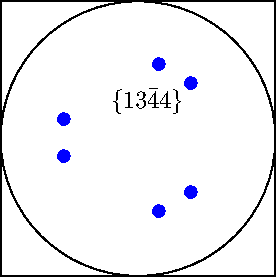
\includegraphics[width=3cm]{pic/miller}
%   \end{column}
% \end{columns}


% 	\begin{onlyenv}<2>

% 		\lstset{stringstyle=\color{red},emph={antipodal},emphstyle=\em\color{red}}

% \begin{lstlisting}
% get(h,'hkl')
% eq(h1,h2,`antipodal`), angle(h1,h2,`antipodal`)
% symmetrise(h,`antipodal`)
% plot([h1,h2],'all',`antipodal`)
% \end{lstlisting}


%     \end{onlyenv}


% \end{frame}



% \begin{frame}[fragile]
%   \frametitle{Orientations - The \MTEX Class \texttt{\bf orientation}}

% Definition:

% \begin{lstlisting}[mathescape=true]
% ori = orientation(rot,CS,SS)
% ori = orientation('Euler',$\phi_1$,$\Phi$,$\phi_2$,CS,SS)
% ori = orientation('Euler',$\alpha$,$\beta$,$\gamma$,'ABG',CS,SS)
% ori = orientation('Miller',[h k l],[u v w],CS,SS)
% ori = orientation('brass',CS,SS)
% \end{lstlisting}

% \begin{columns}
%   \begin{column}{8.5cm}

%     Calculations:

% \begin{lstlisting}
% r = ori * h, h = ori \ r
% ori = rot * ori
% \end{lstlisting}

%     Basic Functions:

% \begin{lstlisting}[mathescape=true]
% eq(ori1,ori2), angle(ori1,ori2)
% symmetrise(ori), angle(ori)
% project2FundamentalRegion(ori,ref_ori)
% [$\phi_1$,$\Phi$,$\phi_2$]  = Euler(ori)
% \end{lstlisting}

%   \end{column}

%   \begin{column}{3cm}
%     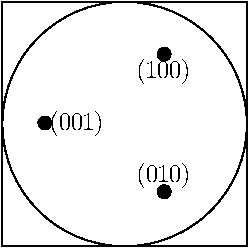
\includegraphics[width=3cm]{pic/quaternion}
%   \end{column}

% \end{columns}
% \end{frame}



\section{Exercises}

\begin{frame}

  \begin{Exercise}
    Consider trigonal crystal symmetry.

  \begin{enumerate}[a)]
    \item Find all crystallographic directions symmetrically equivalent to $h
      = (1, 0, \bar 1, 0)$ (Miller indices)!
    \item Find crystallographic directions such that the number of their
      crystallographic equivalent directions on the upper hemisphere (without
      equator) is 1, 3, and 6, when including antipodal symmetry!
    \item Consider the orientation given by the Euler angles $(30\degree,
      90\degree, 90\degree)$ in Bunge convention. Give the Euler angles of
      all symmetrically equivalent orientations!
    \item Which positions in the (0,0,0,1) - pole figure corresponds to the
      above orientation. Which crystal direction is rotated by this
      orientation to the specimen direction (0,0,1)?
    \item Construct an orientation that rotates the crystallographic
      directions $(0,0,0,1)$ and $(2,\bar 1,\bar 1,0)$ onto the specimen
      directions $(1,0,0)$ and $(0,1,0)$, respectively. Describe the rotation
      by axis and angle.
    \end{enumerate}

  \end{Exercise}

\end{frame}

%%% Local Variables:
%%% mode: latex
%%% TeX-master: "main"
%%% End:
